\documentclass[12pt]{article}
 
\usepackage[margin=1in]{geometry}
\usepackage{amsmath,amsthm,amssymb}
\usepackage{fancyhdr}
\usepackage{hyperref}
\pagestyle{fancy}
\usepackage{graphicx}
\newcommand{\N}{\mathbb{N}}
\newcommand{\R}{\mathbb{R}}
\newcommand{\Z}{\mathbb{Z}}
\newcommand{\Q}{\mathbb{Q}}
 
\newenvironment{theorem}[2][Theorem]{\begin{trivlist}
\item[\hskip \labelsep {\bfseries #1}\hskip \labelsep {\bfseries #2.}]}{\end{trivlist}}
\newenvironment{lemma}[2][Lemma]{\begin{trivlist}
\item[\hskip \labelsep {\bfseries #1}\hskip \labelsep {\bfseries #2.}]}{\end{trivlist}}
\newenvironment{exercise}[2][Exercise]{\begin{trivlist}
\item[\hskip \labelsep {\bfseries #1}\hskip \labelsep {\bfseries #2.}]}{\end{trivlist}}
\newenvironment{problem}[2][Problem]{\begin{trivlist}
\item[\hskip \labelsep {\bfseries #1}\hskip \labelsep {\bfseries #2.}]}{\end{trivlist}}
\newenvironment{question}[2][Question]{\begin{trivlist}
\item[\hskip \labelsep {\bfseries #1}\hskip \labelsep {\bfseries #2.}]}{\end{trivlist}}
\newenvironment{corollary}[2][Corollary]{\begin{trivlist}
\item[\hskip \labelsep {\bfseries #1}\hskip \labelsep {\bfseries #2.}]}{\end{trivlist}}
 
\begin{document}
 
\title{Lab 5: Congestion Control for Audio Streaming}
\author{Duc Viet Le\\
 CS536}
 
\maketitle
 
\begin{problem}{1} \ \\
Below are plots for each method:
\\
\textbf{Method A} \\
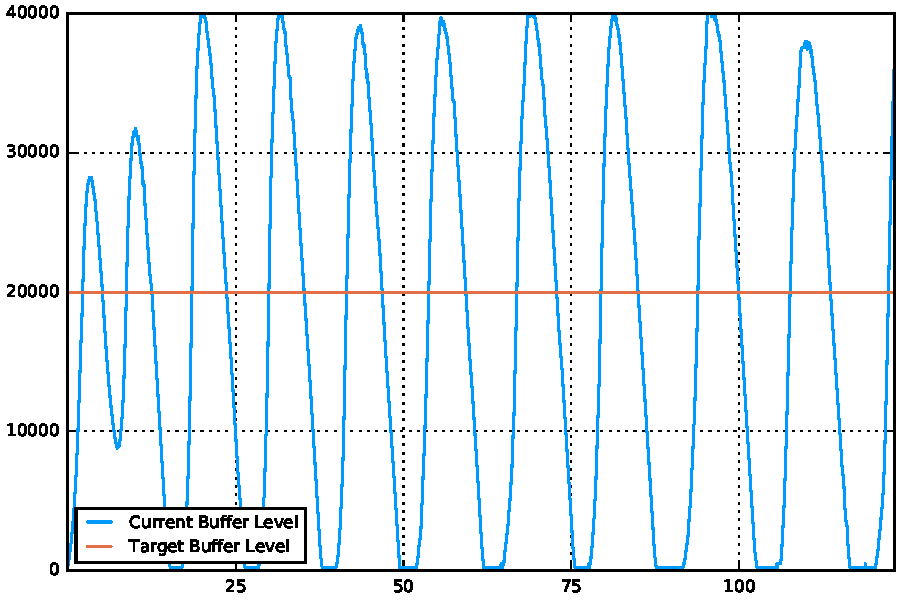
\includegraphics[scale = .5]{listen0.pdf}
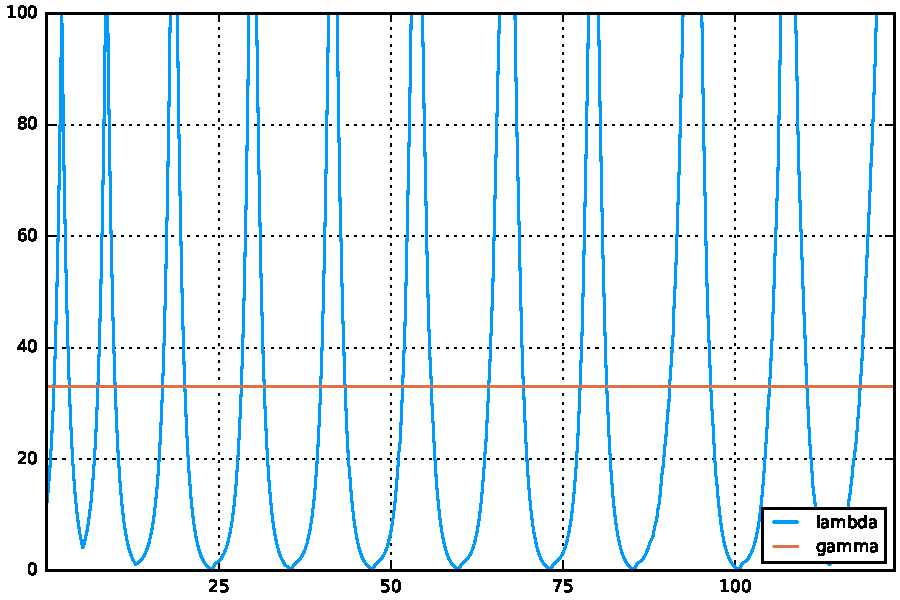
\includegraphics[scale = .5]{stream0.pdf}
\\
\textbf{Method B} \\
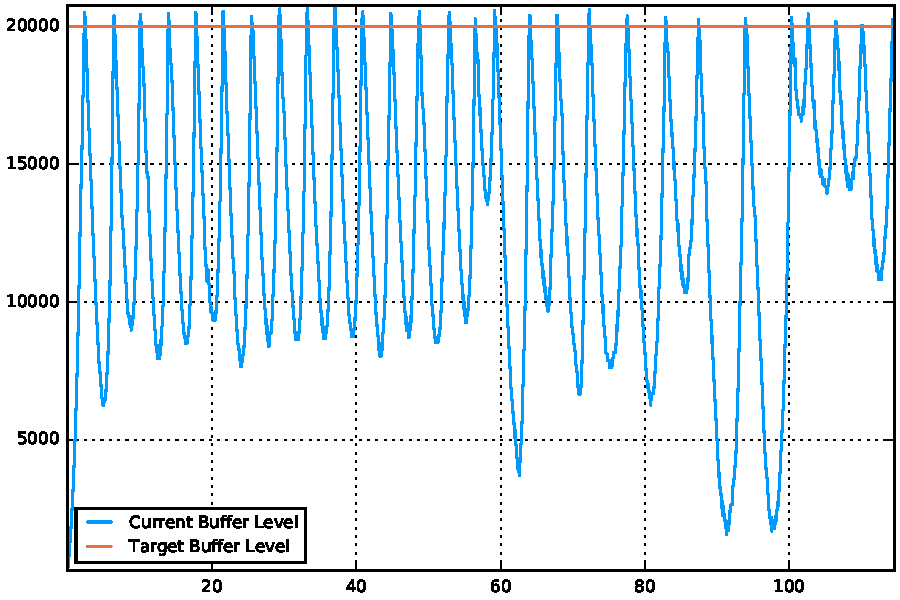
\includegraphics[scale = .5]{listen1.pdf}
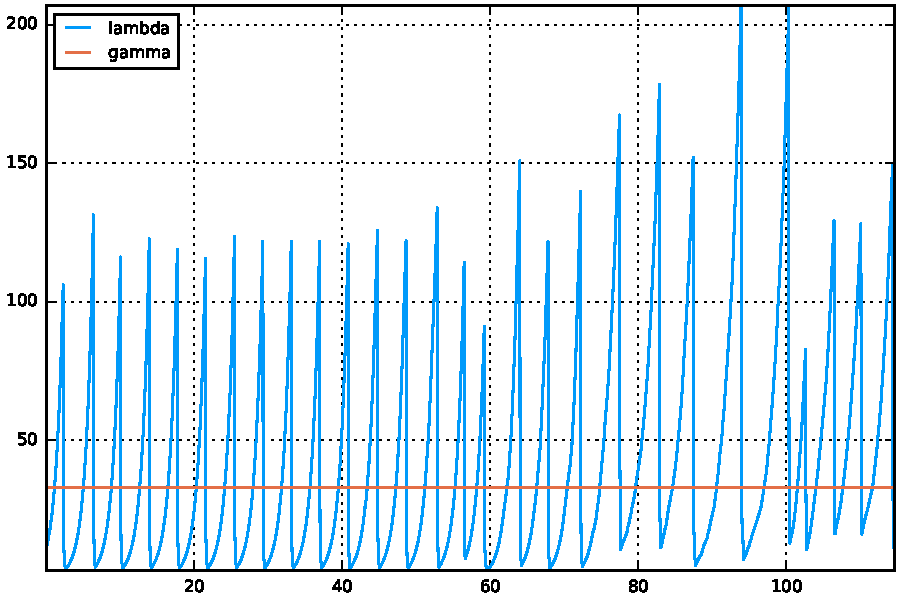
\includegraphics[scale = .5]{stream1.pdf}
\\
\textbf{Method C} \\
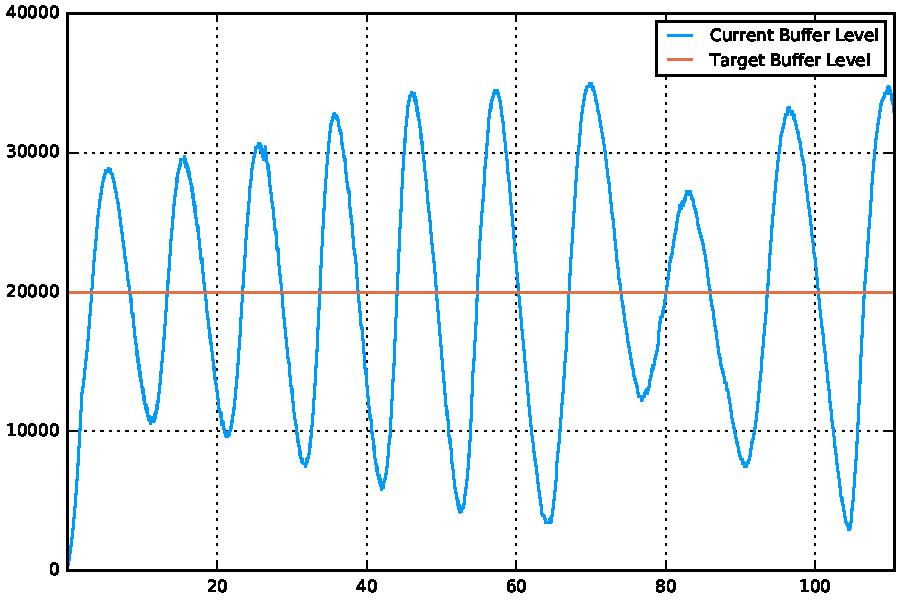
\includegraphics[scale = .5]{listen2.pdf}
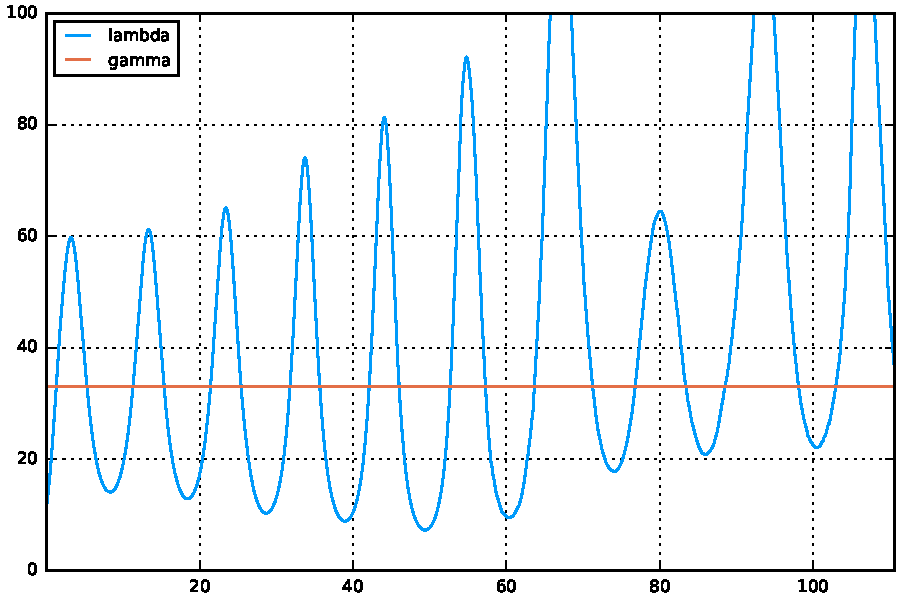
\includegraphics[scale = .5]{stream2.pdf}
\\
\textbf{Method D}
\\
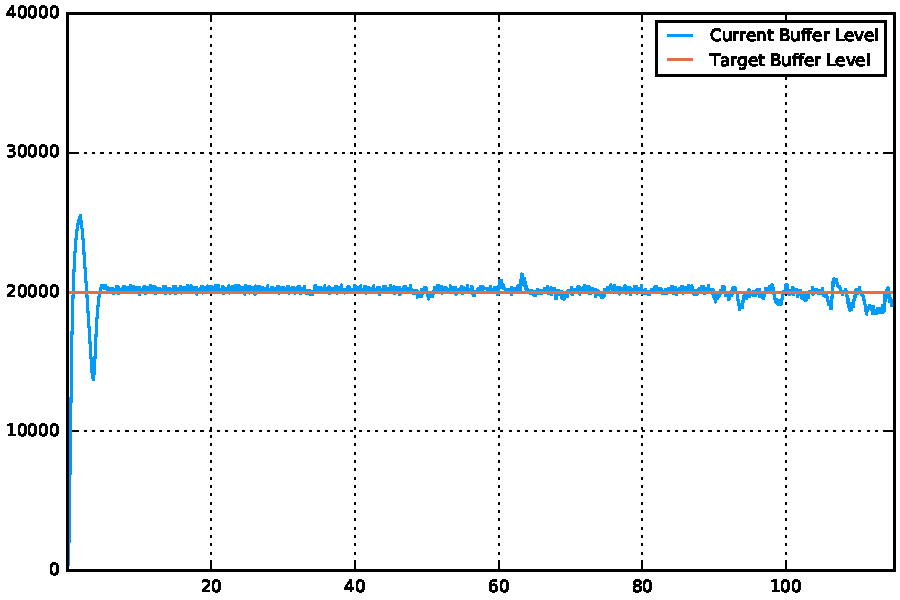
\includegraphics[scale = .5]{listen3.pdf}
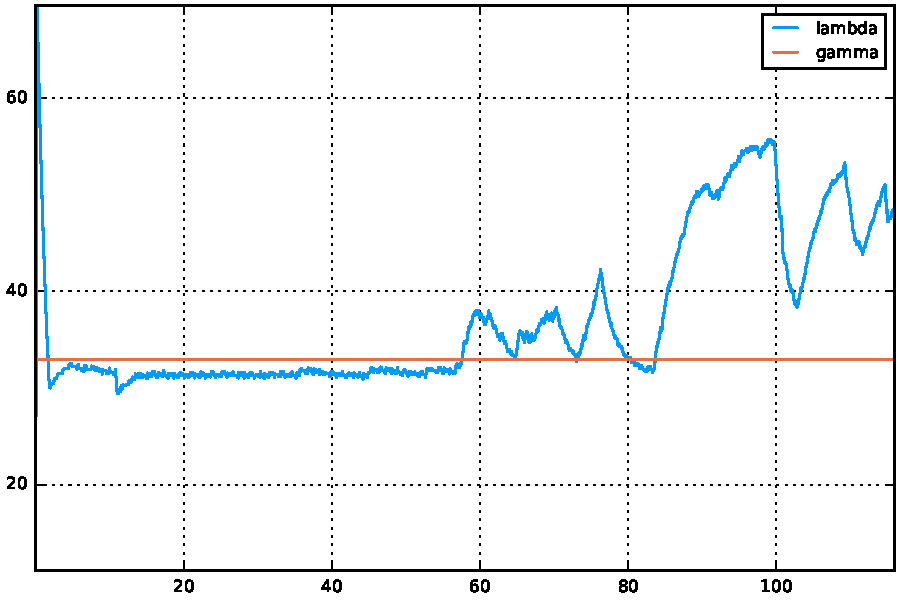
\includegraphics[scale = .5]{stream3.pdf}
\\
\textit{Discussion:}
As we discussed in class, the plot is sample of first 50 seconds of 4 methods. The parameters we used are:
\begin{enumerate}
	\item For method A, $a = 2$
	\item For method B, $a = 2, \delta = 0.5$
	\item For method C, $\epsilon = 0.00005$
	\item For method D, $\epsilon = 0.001, \beta = 0.1$
\end{enumerate}
Method D has the best results and the streaming using method D seems to have better quality. Method B,C also has a decent streaming quality as current buffer level always above payload size. Method A does not have a good streaming quality, as the current buffer level always hits bottom. For testing streaming server with 2 clients, I don't see any significant differences when streaming server supports two clients vs one client.
\end{problem}

\begin{problem}{2}
    For this problem, on client side, I keep track of the sequence number of last package (i.e \texttt{lastPacket}), and compare it with sequence number of incoming package. If the sequence number of new package is greater than the last sequence plus 1, I send a  negative \texttt{ACK}, and update last sequence accordingly. 
    On server side, I store an array that store \texttt{audioBuf} packets and \texttt{packageCounter} that store how many packets sent. If the server receives a negative \texttt{ACK}, it checks if the sequence number is greater than \texttt{packageCount - audioBuf}. If yes, the packet is still in the buffer, the server will retransmit; otherwise, ignore that negative \texttt{ACK}.    
    \\
    Below is graph, using method D:\\
    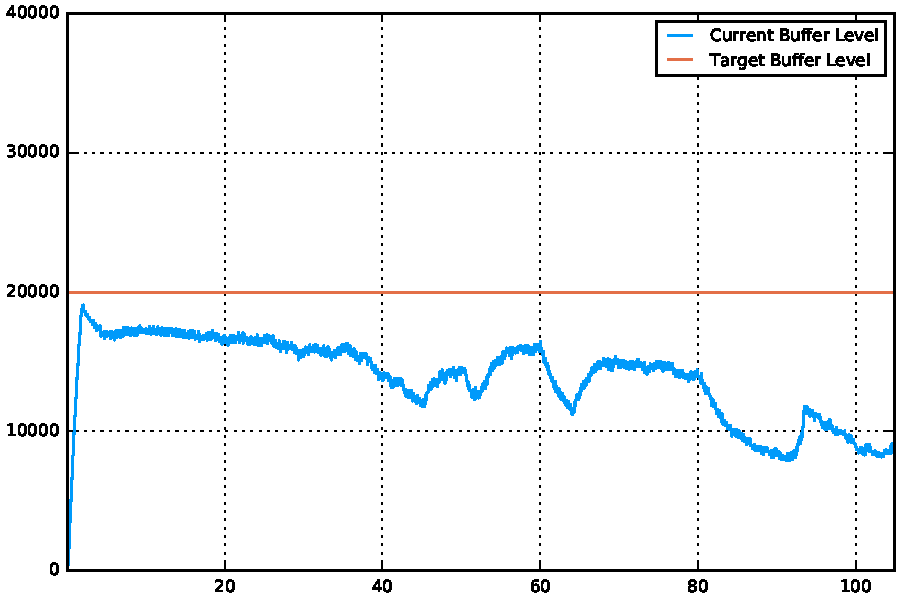
\includegraphics[scale = .5]{q2listen3.pdf}
    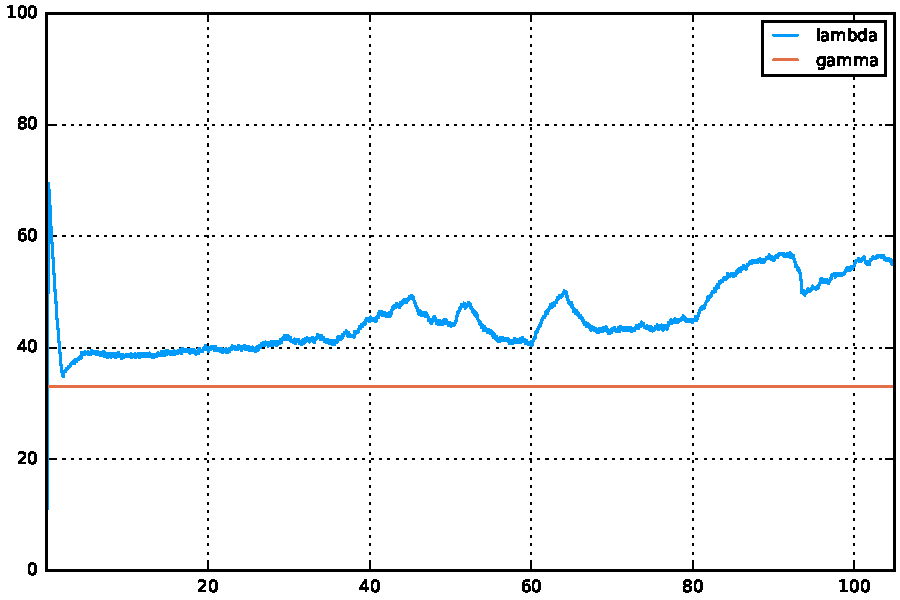
\includegraphics[scale = .5]{q2stream3.pdf}
\end{problem}

\end{document}
